\documentclass[10pt,twocolumn,letterpaper]{article}

\usepackage{cvpr}
\usepackage{times}
\usepackage{epsfig}
\usepackage{amsmath}
\usepackage{amssymb}

\usepackage{booktabs} % for much better looking tables
\usepackage{array} % for better arrays (eg matrices) in maths
\usepackage{paralist} % very flexible & customisable lists (eg. enumerate/itemize, etc.)
\usepackage{verbatim} % adds environment for commenting out blocks of text & for better verbatim
\usepackage{subfigure} % make it possible to include more than one captioned figure/table in a single float
\usepackage{graphicx}

% Include other packages here, before hyperref.

% If you comment hyperref and then uncomment it, you should delete
% egpaper.aux before re-running latex.  (Or just hit 'q' on the first latex
% run, let it finish, and you should be clear).
%\usepackage[pagebackref=true,breaklinks=true,letterpaper=true,colorlinks,bookmarks=false]{hyperref}

\cvprfinalcopy % *** Uncomment this line for the final submission

\def\cvprPaperID{****} % *** Enter the CVPR Paper ID here
\def\httilde{\mbox{\tt\raisebox{-.5ex}{\symbol{126}}}}

% Pages are numbered in submission mode, and unnumbered in camera-ready
\ifcvprfinal\pagestyle{empty}\fi
\begin{document}

%%%%%%%%% TITLE
\title{
Project in CSE 250B\\
Assignment 1: Recognition of Handwritten Digits}

\author{Andreas Landstad, Spencer Bliven, Jonas Hoelzler\\
Computer Science Department\\
University of California, San Diego\\
{\tt\small landstad.andreas@gmail.com, sbliven@ucsd.edu, jonas@hoelzler.de}
}% For a paper whose authors are all at the same institution,
% omit the following lines up until the closing ``}''.
% Additional authors and addresses can be added with ``\and'',
% just like the second author.
% To save space, use either the email address or home page, not both
%\and
%Second Author\\
%Institution2\\
%First line of institution2 address\\
%{\tt\small secondauthor@i2.org}
\maketitle
\thispagestyle{empty}

%%%%%%%%% ABSTRACT
\begin{abstract}
In this in-class project different variants of nearest neighbor classifiers for handwritten digit recognition are implemented and compared. The results are evaluated using the USPS dataset. It was found out that the k nearest-neighbor classification method (kNN) using Euclidean distance yields the lowest error rate of all implementet variants with 5.6\%.
The weighted similarity function is slighly worse with 5.8\% due to overfitting.   
Both results are significantly worse than the best known results with an error rate of 2.2\%.
\end{abstract}

%%%%%%%%% BODY TEXT
\section{Introduction}

\subsection{Nearest Neighbor Classification}
The nearest neighbor classification is a supervised learning method. Given are training examples $\langle x,y \rangle$ where $x$ is an instance and $y$ is a label and test examples which are instances $x$ with unknown labels. The goal is to predict labels for test examples. The nearest neighbor classification method is perhaps the simplest of all supervised learning algorithms. The training phase is no more than storing every training example with its label. To make a prediction for a test example, one has first to compute its distance to every training example. In the $k$ nearest neighbor classification ($k$NN) one has to keep the $k$ closest training examples. On the basis of the $k$ labels of the $k$ nearest neighbors one has to decide for one label. The procedure in this paper therefore is explained in section \ref{kNN}. The second major design step is how to choose the distance function. The design decisions for this project are explained in section \ref{distancefunctions}.
 

\subsection{The USPS dataset}
In this project the algorithms are applied to the multiclass learning problem of recognizing handwritten digits taken from the US Mail (Figure \ref{digits}).

The so called USPS dataset contains training and test data from normalized handwritten digits, automatically
scanned from envelopes by the U.S. Postal Service. The original scanned digits are binary and of different sizes and orientations; the images have been deslanted and size normalized, resulting in 16 x 16 grayscale images \cite{LeCun}. The image instances are represented by a vector with 256 features. Since the effictive dimensionality is much smaller, the curse of dimensionality does not apply. There are 7291 training observations and 2007 test observation. The distribution of the observations is shown in Figure \ref{distribution}.
\begin{figure}[htbp]
  \centering

    \begin{minipage}{8 cm}
      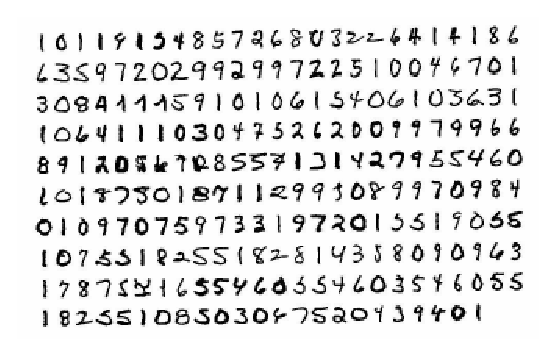
\includegraphics[width=8cm]{digit2}
      \caption{Examples of USPS digits}
      \label{digits}
    \end{minipage}

\end{figure}
\begin{figure*}[tb]
	\centering

 		\begin{tabular}{|l|l|l|l|l|l|l|l|l|l|l|}
  	\hline
  	 ~ & 0 & 1 & 2 & 3 & 4 & 5 & 6 & 7 & 8 & 9 \\ 
  	 \hline
		Training Set  & 0.16 & 0.14 & 0.1 & 0.09 & 0.09 & 0.08 & 0.09 & 0.09 & 0.07 & 0.09 \\ 
		Test Set & 0.18 & 0.13 & 0.1 & 0.08 & 0.10 & 0.08 & 0.08 & 0.07 & 0.08 & 0.09 \\
  	\hline
 		\end{tabular}
\caption{Distribution of the USPS Traing and Test Sets}
    \label{distribution}
\end{figure*}

\section{Design of Algorithms}
The $k$ nearest neighbors, as measured by each distance function, were used to predict the label for each test image. The major design steps are choosing the distance function, choosing how many nearest neighbors are considerd and how to select the most common label of the selected $k$ nearest neighbors.

\subsection{Distance functions}
\label{distancefunctions} 

Choosing a distance function is critical for $k$ nearest neighbors. Ideally, the distance function should always return a very small value for points with the same label and very large numbers for points with different labels. The greater the separation between the intra-label and inter-label distributions, the lower the error rate of the $k$NN algorithm.  To assess the suitability of various distance functions for image processing, $k$NN was trained using the USPS zipcode data.

Five distance functions were considered: Euclidean distance, weighted euclidean distance, similarity, weighted similarity, and manhattan distance. The five functions are summarized in Table~\ref{tab:distfns}.

Euclidean distance (2-norm) and manhattan distance (1-norm) were calculated in the typical manner. Similarity was modified somewhat from the standard dot-product to fit $k$NN. First, all points were normalized to have norm 1. Next, the similarity was calculated by dot-product, yielding a similarity from -1 to 1. To allow $k$NN to operate on this function, we took $1-x\cdot y$, yielding a value in $[0,2]$, where lower values indicate closer points.

Weighted euclidean distance and weighted similarity both required training the weights vector, $w$. This was done by minimizing an objective function via linear regression. 
For weighted similarity, the objective function was to minimize
\[ \sum_{j=1}^N \left( \hat{l}_j - w_0 - \sum_{i=1}^m w_i x_i y_i  \right) ^2  + \lambda \sum_{i=1}^m w_i^2 \]
over all $w$, where $\hat{l}_j$ represents the ideal similarity between $x$ and $y$ and $N$ is the number of $(x,y)$ pairs considered during training. In this case, $\hat{l}_j$ is 1 when the labels for $x$ and $y$ match, and -1 otherwise. As explained above, the USPS training set contains 7291 images. From these, 10000 positive examples of $(x,y)$ with matching labels were chosen at random with replacement, and 20000 negative examples with differing labels were chosen.

Choosing the penalty coefficient, $\lambda$, is a difficult prospect. A range of values for $\lambda$ were tested, with new weights recalculated for each. Each set of weights was used with $k$NN to predict labels for the training set (see Figure \ref{fig:lambda}). Using this procedure we found a value of $\lambda=10$ to be optimal. The weights associated with this $\lambda$ were then used to predict the test images.

For weighted euclidean distance, the objective function was to minimize
\[ \sum_{i=1}^N \left( \hat{l}_j - w_0 + \sum_{i=1}^m w_i (x_i-y_i)^2 \right)\]
over all $w$.
Here determining the ideal distance $\hat{l}$ is more difficult. It was chosen to let $\hat{l} = \sum_{i=1}^m (x_i-y_i)^2 $ for negative examples, and $\hat{l}=0$ for positive samples. This attempts to learn weights such that points with the same label will be close, while the distance between unrelated points will be unchanged. 30000 pairs of points were sampled in the same manner as for weighted similarity, and linear regression again used to determine the optimum weights for the objective function.

\begin{figure}[htbp]
  \centering

    \begin{minipage}{7 cm}
      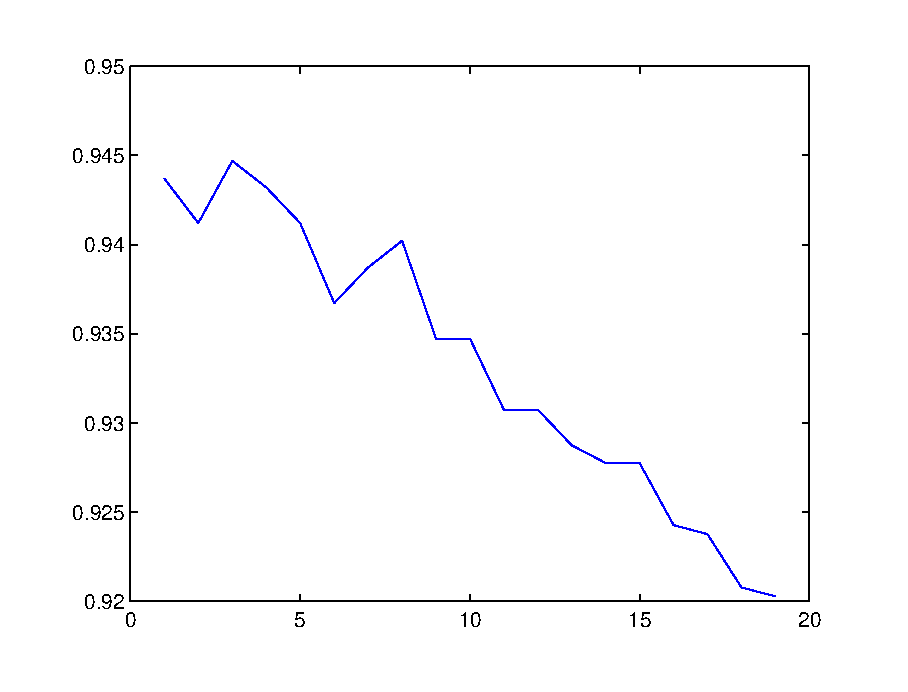
\includegraphics[width=7cm]{kplot}
      \caption{Error rates of kNN using Euclidian distance for different $k$}
      \label{kplots}
    \end{minipage}

\end{figure}



\begin{table*}[htdp]
\begin{center}
\begin{tabular}{ll}
\toprule
\bf{Distance Function} & Formula \\
\midrule
Euclidean & $\left( \sum_{i=1}^m (x_i-y_i)^2 \right) ^{1/2}$ \\
Weighted Euclidean & $ \left( w_0 + \sum_{i=1}^m w_i (x_i-y_i)^2 \right)^{1/2}$ \\
Similarity & $1-\sum_{i=1}^m x'_i y'_i $ \\
Weighted Similarity & $1-\left(w_0 + \sum_{i=1}^m w_i x'_i y'_i \right) $ \\
Manhattan distance & $ \sum_{i=1}^m | x_i-y_i | $ \\
\bottomrule
\end{tabular}
\end{center}
\caption{Overview of the $k$NN with a variety of distance functions. In each case, $x$ and $y$ represent points in $\mathbb{R}^m$, $w$ represents a weight vector in $\mathbb{R}^{m+1}$. Normalized points are expressed as in $x' = \frac{x}{||x||_2}$. }
\label{tab:distfns}
\end{table*}



\subsection{Design of $k$NN classification function}
\label{kNN}
Using a desired distance function, the $k$ nearest neighbours to a test example can be found.

\subsubsection*{Choosing a label}
Given are the $k$ closestes instances with their label and the distance to the test examples.
In this project the label with plurality among the $k$ closest neighbours is selected. If there is no single lable which has a plurality, the label among the plurality-winning labels is selected that has the instance with the closest distance. There can also be a tie here if two or more labels have the exact same distance from the point as well as the the same plurality. Since that is not very likely, one of these labels is selected ranomly.  
\subsubsection*{Choosing $k$}

A small odd integer is selected for $k$, because this reduces the chance of a tie when there are two labels that are overlapping in $\mathbb{R}^m$.
In Figure \ref{kplots} you can see the error rates for different $k$s on the example of the euclidean distance function. Small odd integers result in lower error rates. Selecting bigger $k$s will probably include non-important neighbours that are far from the target.
If $k$ also should not be selected too small ($k=1$). The likelihood of one point from another label being closest to a point that should be labelled with another label is more likely than having more points if some variance for each label and little clustering of the noise is expected. Noise is interpreted as single points that are far from the mean of the rest of the points, i.e., points that in the distribution of lengths from the mean of the points would be in a low percentile. Thus $k=3$ is selected. 

\section{Evaluation}
The performance of the algorithms are compared using the error rate. The error rate of the method is defined as the percentage of labels not correctly predicted. The result are listed in Table \ref{results}. The $k$NN algorithm implemented as explained above performed best using the euclidean distance with 5.6\%. The similarity function distance and the manhattan distance performed worse with 5.8\% respectively 6.3\%. In cases of the euclidean distance and the similarity function weighting led to worse results probably due to overfitting. The results were significantly worse than human performance with 2.5\%. There are some other algorithms which are better. The Covariance Support Vector Machine (\cite{shivas} performed better with 4.3\%. In 1993, Simard et al. proposed an invariant distance measure called tangent distance \cite{Simard}. The authors observed that reasonably small transformations of certain image objects does not affect class membership. Simple distance measures like the Euclidean distance do not account for this, instead they are very sensitive to affine transformations like scaling, translation, rotation or axis deformation. The tangent distance leads to better result with 2.5\%, using 9707 instead of 7291 training examples. The best known result for 7291 training examples is based on kernel densities using the tangent distance resulting in 2.2\% \cite{keysers}.   


\begin{figure}[htbp]
\begin{center}
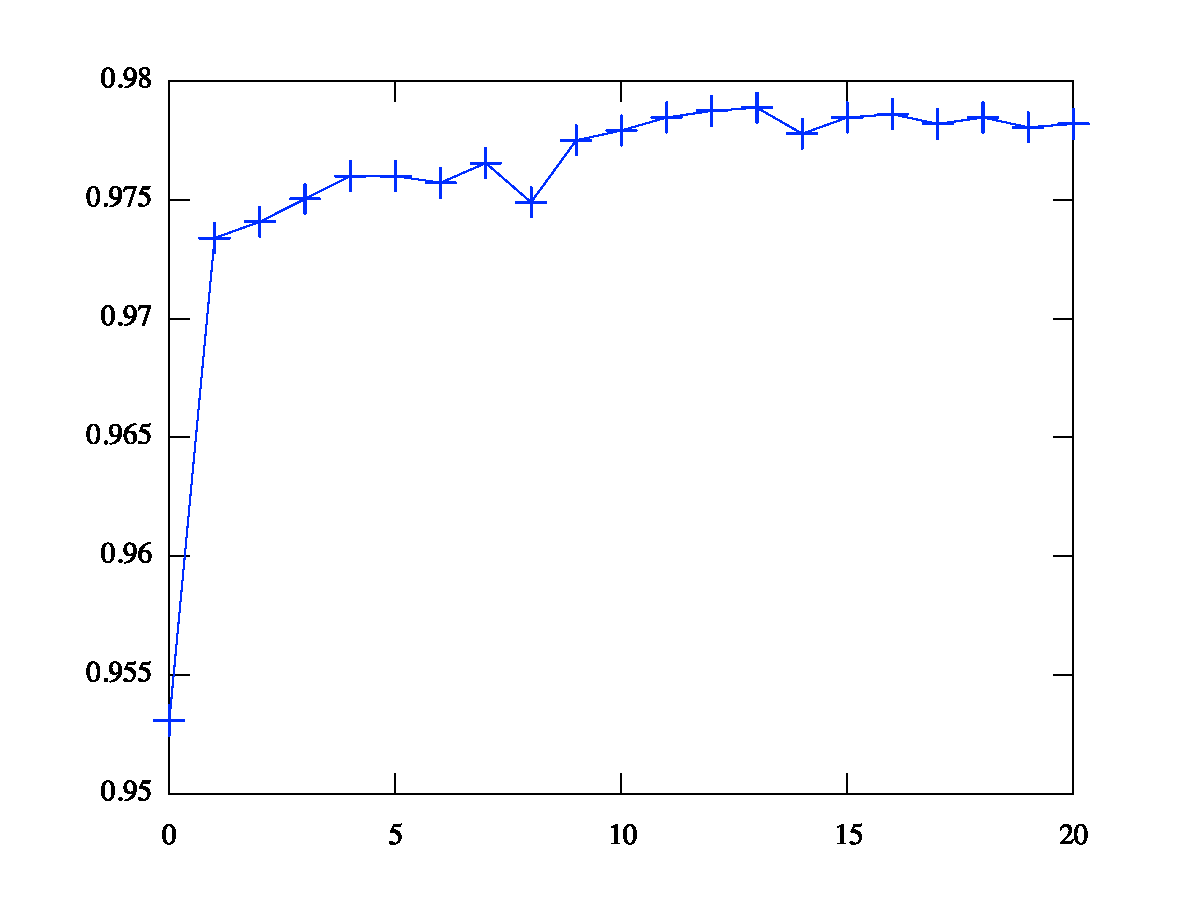
\includegraphics[scale=.5]{weightedSimilarityAccuracy}
\caption{{\bf Error rates of $k$NN using weighted similarity with various values of $\lambda$. $\lambda$ is on the x-axis, error rate on the y-axis.}}
\label{fig:lambda}
\end{center}
\end{figure}


\begin{table*}[htdp]
\begin{center}
\begin{tabular}{llc}
\toprule
\bf{Method} & \bf{Distance function} & \bf{Error rate} \\
\midrule
Kernel Densities \cite{keysers} & Tangent distance & 2.2\% \\
Tangent distance \cite{Simard2}& Tangent distance& 2.5\%* \\
Human Performance \cite{Simard} & - & 2.5\%\\
Covariance Support Vector Machine \cite{shivas} & - & 4.3\%\\
$k$NN & Euclidean distance & 5.6\% \\
$k$NN & Similarity  & 5.8\% \\
$k$NN & Manhattan distance & 6.3\% \\
$k$NN & Weighted Similarity  & 6.7\% \\
$k$NN & Weighted Euclidean  & 7.7\% \\
\bottomrule
*obtained with larger dataset
\end{tabular}
\end{center}
\caption{Summary of results for the USPS dataset. Error rate of selected methods and implemented $k$NN methods with a variety of distance functions. The error rate is measured as the percentage of wrong classified test points by the algorithm. }
\label{results}
\end{table*}

%------------------------------------------------------------------------

\section{Conclusions}
Of the five distance functions implemented, euclidean distance seems to be the best suited for clustering digit images by $k$NN. %However, all distance functions were able to identify digits with high accuracy.
Weighting slightly decreases the accuracy of $k$NN for both euclidean distance and similarity. This may be the result of overfitting.

\section{TODO}
Spencer: Graphics of error rate and not of accuracy
Extend Conclusions
Jonas: Some references are wrong.

\nocite{shivas, elkan, bishop}

{\small
\bibliographystyle{ieee}
\bibliography{egbib}
}

\end{document}
